\documentclass{article}

\usepackage{amsmath}
\usepackage{graphicx}
\usepackage[parfill]{parskip}

\begin{document}
1) Signature a) should be implemented. First, the equals() method should be public 
otherwise the contains() method of ArrayList class is not able to use it. Second, 
all instances of Object class should be a parameter of equals() method. Some might 
argues that only instances of Song class should be a parameter of equals() method 
since the contains() method checks whether if a song with a specific title is in 
the collection. Doing so might cause runtime expcetion when a non Song class object
try to use contains() method. For instance, during the comparison, the equals() method 
will access the attribute, which stores the title of the song but non Song class 
object do not have this attribute.

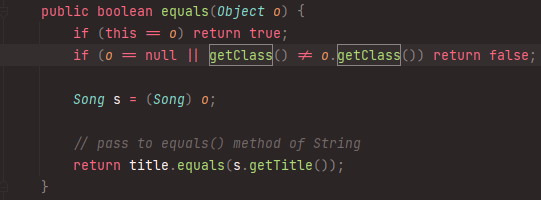
\includegraphics[width=\textwidth]{snippet.PNG}

4) According to the current implementation of class Album, null will not to be added to 
an Album. null will be identified before passing into contains() method. Without doing 
this conditional check, null will be added to Album after passing it to equals() 
via contains() method since equals() will return ``false''. The reason why equals
() method does not complain about this is that this method itself only check 
whether if two Song objects have the same title. If one of objects is not a Song 
objects or null, it will return ``false'' because objects from different classes 
cannot compare to each other, otherwise, it will rise exceptions.

5) There are issues with allowing null to be added to an Album. When the Album 
class or the SongCollection class have some actions related to the attributes 
and methods of the Song objects, and these actions apply to null, it will give
 rise of exceptions becasue null is not an object nor an Song object neither, 
 which means that it does not contain anything attributes and behaviour.

\end{document}